% Methods section, city square exposure at 15 GHz.
% Build: pdflatex methods && pdflatex methods
\documentclass[journal]{IEEEtran}

\usepackage[T1]{fontenc}
\usepackage{amsmath,amssymb}
\usepackage{graphicx}
\usepackage{booktabs}
\usepackage{algorithm}
\usepackage{algpseudocode}
\usepackage[hidelinks]{hyperref}
\usepackage{cleveref}

% IEEE abbreviates figure and table references in running text.
\crefname{figure}{Fig.}{Figs.}
\Crefname{figure}{Fig.}{Figs.}
\crefname{table}{Table}{Tables}
\crefname{algorithm}{Algorithm}{Algorithms}

\graphicspath{{../FIGURES/}}

\newcommand{\uloc}{\hat{u}}
\newcommand{\uext}{\hat{v}}
\newcommand{\nhat}{\hat{n}}
\newcommand{\khat}{\hat{k}}
\newcommand{\x}{\mathbf{x}}
\newcommand{\dOmega}{\,\mathrm{d}\Omega}

\begin{document}

\title{Exposure of a pedestrian in a city square at 15\,GHz: method}
\author{Robin~Wydaeghe%
\thanks{The author is with the Department of Information Technology, Ghent
University / imec, 9052 Ghent, Belgium.}}

\maketitle

\section{Exposure ratio}

A person standing in a city square receives radio power from many base stations
at once. The buildings around them block part of that power and reflect part of
it back, so the total depends on the shape of the square as much as on any
single antenna. This paper computes that dependence as one number,
\begin{equation}
  \chi = \frac{S}{S_0} ,
  \label{eq:chidef}
\end{equation}
where $S$ is the power density arriving at the head in the real square and $S_0$
is the power density the same network would deliver at the same point over open
ground. We call $\chi$ the exposure ratio.

The ratio is the useful quantity because the network is unknown. An absolute
exposure in W/m$^2$ needs the transmit power, the number of sites and their
positions, none of which is public at millimetre wave frequencies and none of
which is a property of the square. Dividing by the free space answer removes all
three. What is left is a pure number that is 1 when the square is empty, below 1
where the buildings shadow more than they reflect, and above 1 where they
reflect more than they shadow. It transfers between cities, which a power
density does not.

Computing $\chi$ directly would mean placing a transmitter at every position a
base station could occupy and tracing rays from each one to the person. That is
the expensive way round. Instead everything is computed at the one point where
the person stands. Rays are launched from that point, followed until they leave
the square, and weighted by how likely a base station is to sit in the direction
each one left. \Cref{fig:adjoint} shows the idea. One trace per standpoint then
answers the question for every base station position at once.

Putting the transmitter and the receiver at the same point is what makes the
rest of the method possible, because a street level photograph taken from that
same point sees the surfaces the early bounces will hit. The material of a
facade is therefore measured rather than assumed, and how far that measurement
reaches is what sets how many bounces are worth following.
Section~\ref{sec:budget} returns to this and fixes the bounce budget from it.

\begin{figure}[!t]
  \centering
  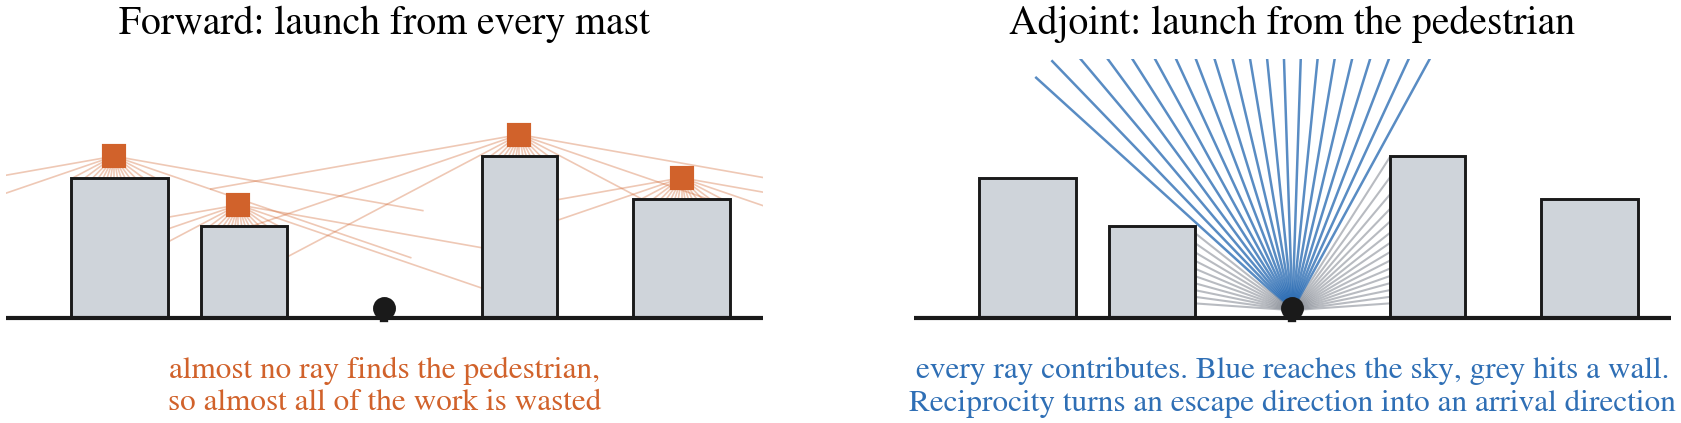
\includegraphics[width=\columnwidth]{20_adjoint_idea.pdf}
  \caption{Rays are shot outward from the person rather than inward from the
  sources. A path is reversible, so a ray that leaves in direction $\uloc$ and
  escapes the square in direction $\uext$ carries the same attenuation as a ray
  arriving from a source in direction $\uext$ and reaching the person from
  direction $\uloc$.}
  \label{fig:adjoint}
\end{figure}

\subsection{Notation}

Vectors are boldface, unit vectors carry a hat. $\uloc$ is a direction leaving
the observation point and $\uext$ is the direction in which a ray finally
escapes. Angles are measured from the horizon upward, so $\alpha$ is elevation
and $\alpha = 0$ is level with the head. \Cref{tab:symbols} lists the symbols
used in the equations.

\begin{table}[!t]
  \caption{Symbols}
  \label{tab:symbols}
  \centering
  \begin{tabular}{llc}
    \toprule
    Symbol & Meaning & Unit \\
    \midrule
    $\x$ & observation point, the head of the pedestrian & m \\
    $\uloc$ & direction leaving $\x$ & -- \\
    $\uext$ & direction in which a ray escapes the scene & -- \\
    $\alpha$ & elevation above the horizon & rad \\
    $r$ & horizontal range from $\x$ to a site & m \\
    $\rho$ & slant range from $\x$ to a site & m \\
    $h$ & height of a site above $\x$ & m \\
    $\nu$ & number of sites per unit volume & m$^{-3}$ \\
    $Q(\uext)$ & share of incident power per steradian of sky & sr$^{-1}$ \\
    $\Phi(\uloc)$ & power arriving per steradian, in units of $S_0$ & sr$^{-1}$ \\
    $S$, $S_0$ & arriving and free space power density & W/m$^2$ \\
    $\chi$ & exposure ratio, $1$ in free space & -- \\
    $w$ & power carried by one ray, $1$ at launch & -- \\
    $\Gamma$ & Fresnel reflection coefficient & -- \\
    $\kappa$ & fraction of reflected power that stays specular & -- \\
    $\sigma_h$ & root mean square surface roughness & m \\
    $\varepsilon_r$ & complex relative permittivity & -- \\
    $\lambda$ & wavelength & m \\
    $N$ & rays launched per standpoint & -- \\
    $M$ & cells in the launch grid & -- \\
    $L$ & largest number of surface interactions & -- \\
    $S_{ab}$ & absorbed power density on the body & W/m$^2$ \\
    $T_0$ & power transmitted into tissue at normal incidence & -- \\
    $\nhat$ & outward normal of a body facet & -- \\
    $\khat$ & propagation direction of an incident wave & -- \\
    \bottomrule
  \end{tabular}
\end{table}

\subsection{Assumptions}

The method rests on seven assumptions, stated here because each one bounds what
the results can mean.

\begin{enumerate}
  \item[A1] \emph{Far field.} Every source is far enough away that it
  illuminates the square with a plane wave. The nearest site considered is
  25\,m from the head, and the array apertures involved are under 0.3\,m, so
  this holds throughout.
  \item[A2] \emph{Powers add, phases do not.} Contributions from different
  paths are summed in power. At 15\,GHz and a 100\,m range, the phase of a path
  turns by about $3.1 \times 10^{4}$\,rad per radian of change in the exit
  angle, so resolving it would need on the order of $10^{10}$ angular cells
  against the 512 used here. Any phase this method could carry would be noise.
  \item[A3] \emph{Sites are a density, not a list.} Base station positions are
  unknown and are modelled as a uniform density over a slab of ground, bounded
  in height and in range. Section~\ref{sec:illum} builds the model.
  \item[A4] \emph{Every site delivers the same power at the head.} Sites are
  counted rather than weighted by their range, so the angular distribution of
  incident power follows the angular distribution of site count. A variant that
  weights each site by its own free space spreading is reported alongside.
  \item[A5] \emph{Surfaces are locally flat.} Each triangle is treated as a
  smooth interface with a Gaussian height error of standard deviation
  $\sigma_h$ about its own plane.
  \item[A6] \emph{No diffraction.} Energy bending around building edges is
  absent. The paragraph after this list gives the reason and the direction of
  the resulting error.
  \item[A7] \emph{Unpolarised.} Reflection uses the average of the two
  principal polarisations rather than tracking a polarisation state.
\end{enumerate}

A6 is the assumption a reader is most likely to challenge, so it is worth the
space. Three things make it defensible at this frequency and for this quantity.

The first is scale. The wavelength at 15\,GHz is 2\,cm, and the strength of a
diffracted field relative to the field that produced it falls off as
$1/\sqrt{ks}$ with distance $s$ from the edge. At 10\,m that ratio is about
$1/56$ in amplitude, near 35\,dB down in power. Diffraction is a correction to a
picture that reflection already describes, which is the opposite of its role at
the metre wavelengths where street models were first built and where an edge is
only a few wavelengths away from everything.

The second is where that correction would actually lead. Diffraction dominates
only in deep shadow, at points no direct or reflected path reaches, and the
standpoints used here are required to have open sky above them. Points with no
sky are discarded before any trace runs. No standpoint sits in the regime where
the omitted term is the leading one.

The third is that the error has a known sign. A diffracted path can only deliver
power the trace does not currently collect, never remove any, so leaving it out
biases $\chi$ low. Every value reported here is a lower bound with respect to
this term, and the shortfall grows with how narrow and how enclosed the street
is. That is the right direction for an omission to run in an exposure study, and
it is stated rather than assumed away.

The remaining sections describe the scene, the illumination model, the ray
estimator, the body, and the checks that constrain them.

\section{Configuration}

The scene is a photogrammetric mesh of a real square, cut to a cylinder of
radius 250\,m about the standpoint and reaching from the ground to the roofline.
The mesh comes from aerial and street level imagery and carries no material
information of its own, so classes and electromagnetic parameters are assigned
afterwards. Radius 250\,m is not a free choice and Section~\ref{sec:valid}
reports what sets it.

\subsection{Surfaces and materials}

Every triangle is assigned one of a small set of classes. In the baseline run
the class follows from geometry alone, splitting near horizontal faces at ground
level from near vertical faces above it, with vegetation separated by its
surface roughness at the mesh scale. Each class carries a complex relative
permittivity from the ITU building materials recommendation \cite{itu2040} at
15\,GHz and a root mean square roughness $\sigma_h$ from published surface
metrology on the corresponding material.

An optional path replaces the geometric class with one read from street level
photographs. Panoramas are segmented, registered to the mesh by matching the
skyline they see against the skyline the mesh casts, and their labels are
projected onto the triangles each panorama can see. Two models are used and they
answer different questions. A semantic segmentation network trained on street
scenes names the object, which separates a building from a tree from a road
surface but has one class for every facade regardless of what it is made of. A
promptable segmentation model is then asked for the material within those facade
regions, which is the axis the first model cannot resolve \cite{sam}. The
registration and projection are described in the supplementary information.

Imagery comes from two providers and the split matters when reading coverage.
Sites represented by a single panorama use one provider's official captures,
while the multi-station route at the reference site comes from a second,
community sourced provider, which is the only set carrying the material axis.
The comparison between the geometric and the image derived assignment is a
result rather than part of the method, so it is reported separately.

\subsection{Standpoints}

Exposure is not evaluated at one point. Each site contributes 80 standpoints and
results are reported as a distribution over them rather than as a single value,
because the spread within one square is comparable to the spread between
squares, so a single point would hide most of the variation.

Where a person can stand is decided from the mesh and not from a map. A grid of
columns at 3\,m spacing is laid over the crop, a ray is dropped down each one,
and the column is kept when it lands on a near horizontal face at the square's
ground level with enough clearance that a head at that position is not inside a
wall or a stall. Kept columns are then chained by nearest neighbour, which fixes
an order for plotting and for the step statistics but has no effect on any
exposure value, since each standpoint is traced independently. No street
centreline, footway polygon or other map layer is used, so the sampling does not
inherit whatever a mapping provider decided a street is.

This set of standpoints is distinct from the route the photographs were captured
along, and the two should not be confused. The capture route is wherever the
imagery provider drove or walked, and it determines what the panoramas see. The
standpoints are where exposure is evaluated. They overlap but are neither equal
nor derived from one another.

\section{Illumination model}
\label{sec:illum}

We do not know where the base stations are, so we integrate over where they
could be. Operators do not place millimetre wave sites at arbitrary heights and
ranges: a site sits either on a roof or on street furniture, and beyond some
range its contribution stops mattering. Those two facts bound the region a site
can occupy, and what this section builds from that region is the one function the
estimator needs, the share $Q(\uext)$ of the incident power that reaches the head
from each steradian of sky.

\subsection{Sites per steradian}

Take sites spread uniformly through a slab, with $\nu$ sites per unit volume, at
heights between $h_{\min}$ and $h_{\max}$ above the head and at horizontal
ranges between $r_{\min}$ and $r_{\max}$. Look outward from $\x$ in a direction
at elevation $\alpha$, along a narrow cone of solid angle $\dOmega$. The number
of sites in that cone is the number in the part of it that lies inside the slab
and inside the range band,
\begin{equation}
  \mathrm{d}N = \nu \dOmega \int_{\rho_-(\alpha)}^{\rho_+(\alpha)} \rho^2 \,
  \mathrm{d}\rho
  = \frac{\nu}{3} \left[ \rho_+^3(\alpha) - \rho_-^3(\alpha) \right] \dOmega .
  \label{eq:cone}
\end{equation}
A site at slant range $\rho$ and elevation $\alpha$ has height $\rho \sin\alpha$
and horizontal range $\rho \cos\alpha$, so each band clips the cone from one
side,
\begin{align}
  \rho_-(\alpha) &= \max\!\left( \frac{h_{\min}}{\sin\alpha},
  \frac{r_{\min}}{\cos\alpha} \right), \nonumber \\
  \rho_+(\alpha) &= \min\!\left( \frac{h_{\max}}{\sin\alpha},
  \frac{r_{\max}}{\cos\alpha} \right).
  \label{eq:caps}
\end{align}
\Cref{fig:elevation} draws the geometry behind \eqref{eq:cone}.

What the estimator needs is not a count of sites but a share of incident power.
Under A4 the two are the same function up to a constant, because every site
contributes equally, so
\begin{equation}
  Q(\uext) \;\propto\; \rho_+^3(\alpha) - \rho_-^3(\alpha)
  \label{eq:Q}
\end{equation}
wherever $\rho_+ > \rho_-$, and $Q = 0$ elsewhere. Only elevation appears,
because a uniform density of sites on level ground has nothing to distinguish one
compass bearing from another. Counting sites rather than weighting them by range
is what makes $r_{\max}$ load bearing: the $\rho^2$ inside \eqref{eq:cone} says
far sites are the numerous ones, so where the range band ends decides how much of
the answer they own. Weighting each site by its own free space spreading
$1/\rho^2$ instead replaces the cubed bracket in \eqref{eq:Q} with
$\rho_+ - \rho_-$, and that variant is carried through as a sensitivity.

\begin{figure}[!t]
  \centering
  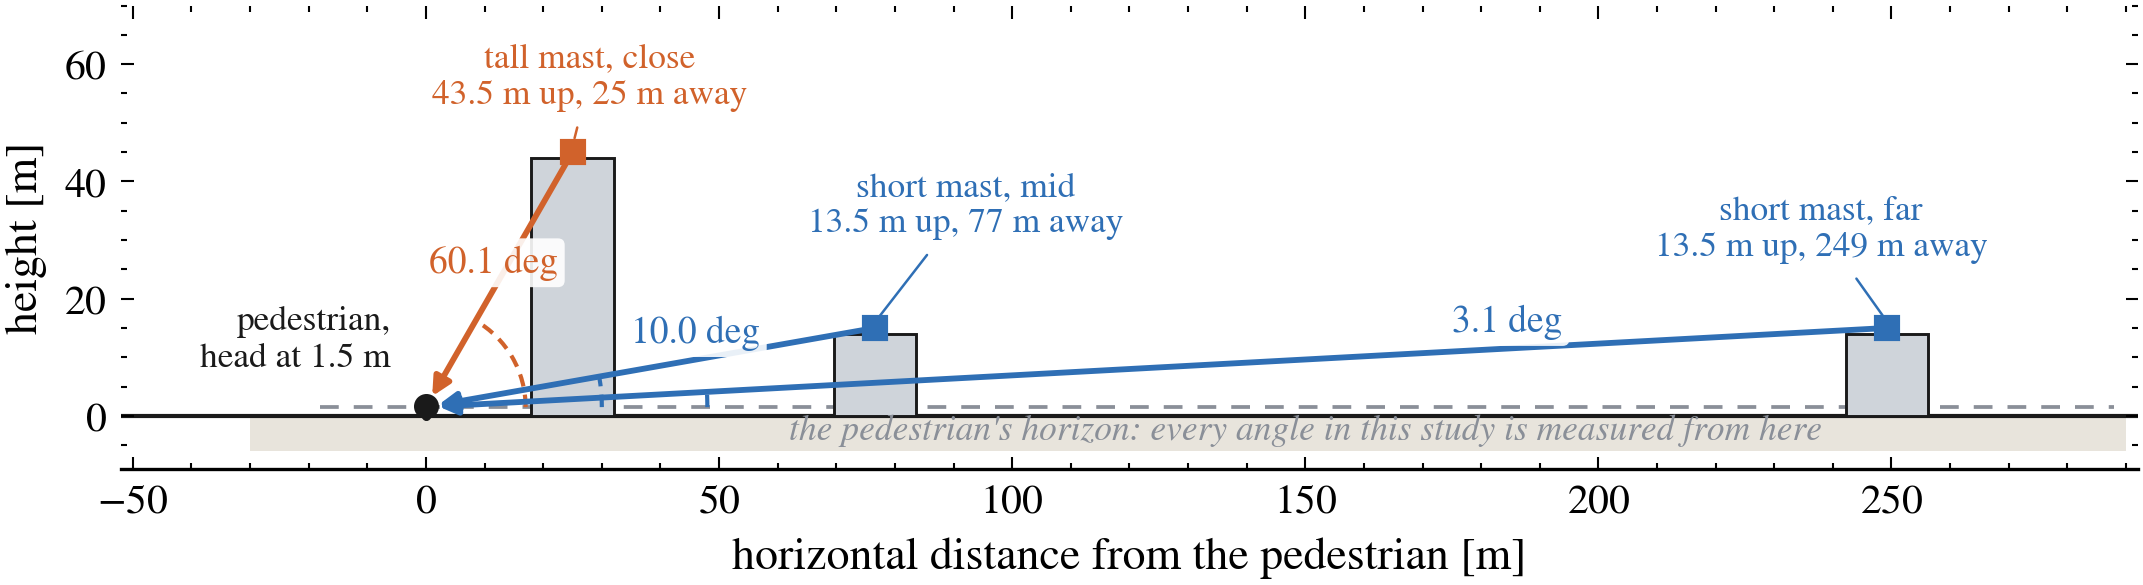
\includegraphics[width=\columnwidth]{18_elevation_geometry.pdf}
  \caption{A site at horizontal range $r$ and height $h$ above the head is seen
  at elevation $\alpha$ with $\tan\alpha = h/r$. Near sites appear high in the
  sky and far sites appear near the horizon, so a band of heights and a band of
  ranges together fix which elevations can hold sites at all.}
  \label{fig:elevation}
\end{figure}

Two consequences follow directly and both matter. First, the support is not a
free parameter. A direction can hold a site only when $\rho_-(\alpha) \le
\rho_+(\alpha)$, which gives
\begin{equation}
  \arctan \frac{h_{\min}}{r_{\max}} \;\le\; \alpha \;\le\;
  \arctan \frac{h_{\max}}{r_{\min}} ,
  \label{eq:support}
\end{equation}
so writing down a height band and a range band already fixes the elevation
limits. Second, the near horizon carries most of the measure, and the near
horizon is also where the buildings act: a distant site sits low in the sky, so
its path grazes along the street and a single facade can intercept it. A site
overhead has no facade in the way. This is why the shape of the square changes
the answer at all, and it is also why the crop radius of Section~II has to be
justified rather than chosen. \Cref{fig:box} shows the region in the height and
range plane.

\begin{figure}[!t]
  \centering
  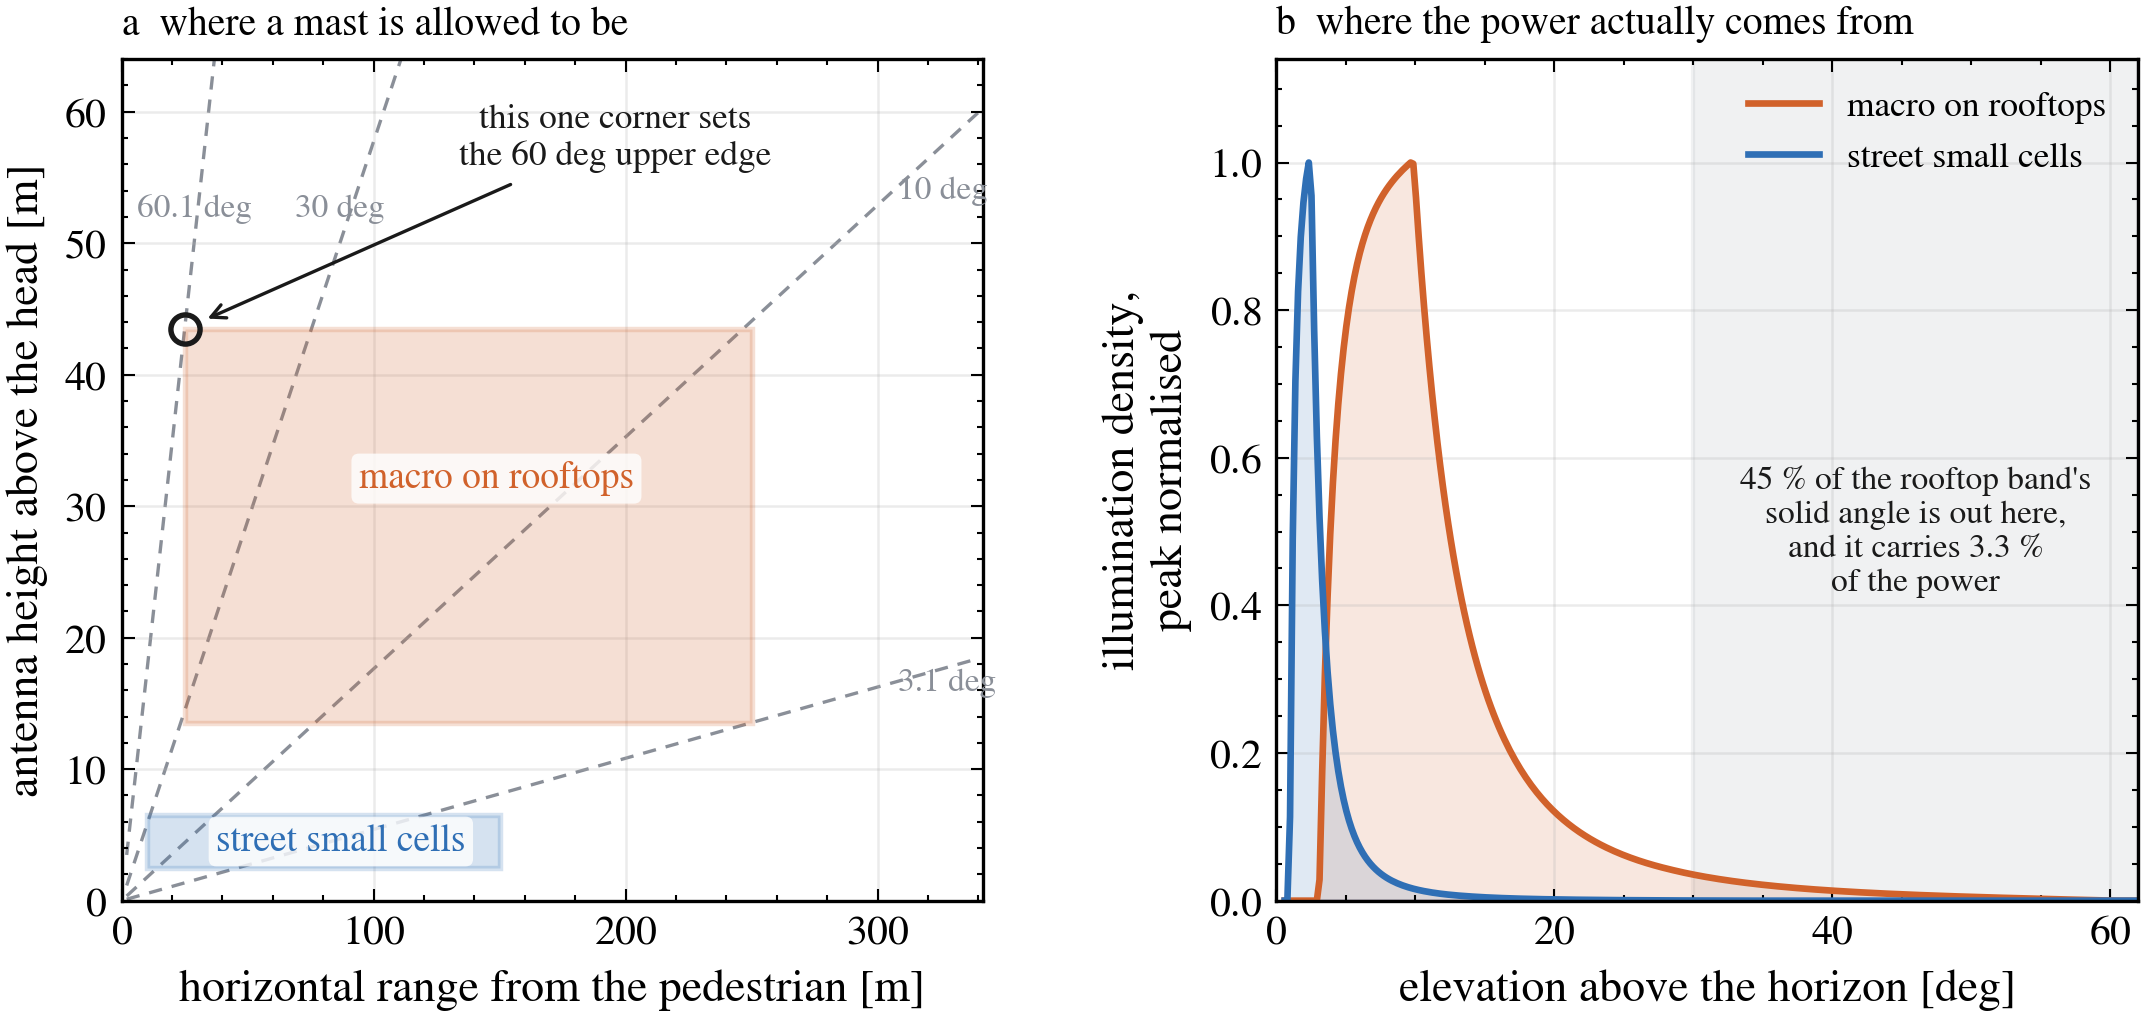
\includegraphics[width=\columnwidth]{19_deployment_box.pdf}
  \caption{The region a site may occupy, in height above the head against
  horizontal range. Lines of constant elevation are straight through the origin,
  so the corners of the box set the elevation limits of \eqref{eq:support}.}
  \label{fig:box}
\end{figure}

\subsection{Normalisation}

$Q$ is scaled so that it integrates to one over the sphere,
\begin{equation}
  \oint Q(\uext) \dOmega = 1 ,
\end{equation}
which is what makes $\chi$ dimensionless and equal to 1 in free space. The
integral is evaluated in elevation rather than on the ray grid, because
$Q$ concentrates within a few degrees of the horizon and a few hundred
grid cells cannot resolve that. The two elevations at which \eqref{eq:caps}
changes branch are inserted into the quadrature abscissae so that no interval
straddles a kink.

\subsection{Models used}

Three illumination models are carried through every run. Their parameters are in
\cref{tab:models}. The isotropic model is a control rather than a deployment: it
weights all directions equally, so under it $\chi$ is exactly the fraction of
the sphere that is open sky, which makes it a check on the estimator as well as
a reference. The rooftop model covers macro sites on buildings and the street
model covers small cells on lamp posts and facades. Their height bands come from
the two ways operators acquire sites, a roof lease or a street furniture lease,
and published deployment heights are bimodal between them rather than spread
across the gap. Because no cellular deployment above 6\,GHz exists in the
European antenna registers, the band edges are not calibrated against measured
millimetre wave siting, and the sensitivity of $\chi$ to them is reported rather
than assumed.

\begin{table}[!t]
  \caption{Illumination models}
  \label{tab:models}
  \centering
  \begin{tabular}{lccc}
    \toprule
    Model & Height above head (m) & Range (m) & Elevation (deg) \\
    \midrule
    Isotropic & -- & -- & $-90$ to $90$ \\
    Rooftop macro & 13.5 to 43.5 & 25 to 250 & 3.09 to 60.11 \\
    Street cell & 2.5 to 6.5 & 10 to 150 & 0.95 to 33.02 \\
    \bottomrule
  \end{tabular}
\end{table}

\subsection{Beam pointing}

A base station at 15\,GHz is an array, not a point radiator, so a reader will
ask what beamforming does to all of this. It depends only on whether the beam
follows the person, and the case that sounds hardest is the one that changes
nothing at all.

Suppose every site puts its peak on the pedestrian. The gain toward the head is
then the same constant in every direction of the sky, so it multiplies
\eqref{eq:Q} and the normalisation divides it straight back out. $Q$ is not
approximately unchanged, it is the same function, and since the estimator reads
$Q$ only when depositing an escaped ray and never inside a random draw, the
traced $\chi$ comes out bit identical. The same cancellation holds for full
digital maximum ratio transmission, where the expected array gain is again
common to every site. The exposure ratio is therefore invariant to beamforming
that tracks the user, exactly rather than approximately, and no array geometry
needs to be specified to say so.

What does move $\chi$ is radiation that is not aimed at the person. A broadcast
beam carries a fixed electrical downtilt, and a beam serving another user points
somewhere else entirely. In both cases the gain becomes a function of elevation
and no longer factors out of the normalisation, so it reweights
\eqref{eq:Q} instead of cancelling. Since the elevation weighting is what
separates one square from another, a fixed pattern can reorder them, and that
variant is carried alongside the three models above.

\section{Adjoint ray estimator}

Reciprocity lets the trace run backwards. A ray leaving $\x$ in direction
$\uloc$, reflecting off surfaces and finally escaping in direction $\uext$ with
a surviving fraction $w$ of its launch power, describes the same physical path
as a wave arriving from a source at $\uext$ and reaching $\x$ from $\uloc$,
attenuated by the same $w$.

That reversal is what makes \eqref{eq:chidef} computable. A ray launched into
$\uloc$ and escaping into $\uext$ collects from the sources that lie in $\uext$,
which carry a share $Q(\uext)$ of the incident power, and it delivers a fraction
$w$ of it. Averaging over the rays launched into $\uloc$ gives the power arriving
from that direction, in units of $S_0$, and integrating over all launch
directions gives back the ratio itself,
\begin{equation}
  \Phi(\uloc) = \big\langle\, w \, Q(\uext) \,\big\rangle_{\uloc} , \qquad
  \chi = \oint \Phi(\uloc) \dOmega .
  \label{eq:chi}
\end{equation}
Nothing about the sources survives except $Q$, so one outward trace answers
\eqref{eq:chidef} for every source position at once. The free space denominator
$S_0$ never has to be computed, because $Q$ was normalised to make it 1.

\subsection{Estimator}

The sphere of launch directions is divided into $M$ cells of near equal solid
angle using a Fibonacci grid. $N$ rays are launched in uniformly random
directions and each is assigned to the cell $c(j)$ nearest its launch direction,
giving $n_c$ rays in cell $c$. Escaping rays deposit into their launch cell, and
the estimate is the cell mean carried through the quadrature,
\begin{equation}
  \hat{\chi} = \frac{4\pi}{M} \sum_{c=1}^{M} \frac{1}{n_c}
  \sum_{j\,:\,c(j)=c} w_j \, Q(\uext_j) .
  \label{eq:estimator}
\end{equation}
Stratifying by launch cell rather than averaging over all rays at once matters
because $Q$ varies by orders of magnitude across the sphere, so an unstratified
average would be dominated by the few rays that happen to escape near the
horizon. In free space every ray escapes unobstructed with $w = 1$ and
$\uext_j = \uloc_j$, so \eqref{eq:estimator} reduces to a quadrature of $Q$ over
the sphere and returns 1, as it must.

The estimator is stochastic, so every reported value carries a Monte Carlo
standard error, obtained by retracing the same standpoints over disjoint seed
streams rather than estimated from within a single run. Seeds and ray counts are
in the supplementary information.

How large that error is depends strongly on which illumination model is being
evaluated, and the reason is worth stating because it decides how many rays a
result needs. The variance is set by the share of the ray budget that lands
inside the support of $Q$. The isotropic model has support everywhere, so every
ray contributes and the per standpoint error is a few thousandths of a decibel.
The street model crowds its entire mass into the lowest tens of degrees of
elevation, so most rays escape into directions where $Q$ is zero and contribute
nothing, and the per standpoint error is some thirty times larger. Stratifying
the launch directions does not help with this, because the launch direction is
not the escape direction and only the latter is weighted. Reporting a median over
many standpoints does help, by roughly the square root of their number, which is
why a distribution over standpoints is the right unit for a claim and a single
standpoint often is not.

\subsection{Bounce loop}

\Cref{alg:trace} gives the loop and \cref{fig:oneray} follows a single ray
through it. Two steps deserve a word.

Roughness splits the reflection rather than blurring it. At each interaction the
fraction of reflected power that survives as a mirror reflection is the Rayleigh
factor
\begin{equation}
  \kappa = \exp\!\left[ -\left( \frac{4\pi \sigma_h \cos\theta_i}{\lambda}
  \right)^{\!2} \right] ,
  \label{eq:rayleigh}
\end{equation}
and the outgoing direction is drawn as a mirror reflection with probability
$\kappa$ and from a cosine weighted lobe about the normal otherwise
\cite{beckmann}. Choosing one lobe with a probability equal to its share of the
energy needs no compensating weight, because the two cancel. Note the
$\cos\theta_i$ in \eqref{eq:rayleigh}: a surface that scatters at normal
incidence behaves as a mirror at grazing incidence, and this is the only place
where that angle dependence enters.

Rays still travelling after $L$ interactions are dropped, and the power they
were carrying is reported as a share of the total, so the truncation is a
measured quantity rather than an assumption. At the budget used here that share
is the estimator's one known bias, and its sign is fixed: discarding surviving
paths can only make $\chi$ too small, never too large.

\subsection{Bounce budget}
\label{sec:budget}

$L = 3$, and the reason is where the material evidence stops rather than where
the number stops moving. A convergence threshold would be the usual argument and
it is the weaker one, because it says only that the tail is small, not that the
tail is right. The panorama argument says something stronger about the part that
is kept.

The photograph is taken from the observation point, so the surfaces a ray can
reach on its first interaction are exactly the surfaces that photograph sees.
That first hit carries measured material by construction, and the guarantee is
exact rather than probable. Nothing beyond the first hit is guaranteed. A ray
that leaves the first facade travels away from the camera that saw it, and
whether its second interaction lands on an observed surface depends on how much
of the square the walk covered, not on any property of the geometry.

The guarantee would extend to the second interaction only for a path that
returns to where it started, since both ends of a closed loop are visible from
the same viewpoint. That is the co-located picture of Section~I in its strictest
form, and it is worth recording that the outward formulation buys its efficiency
partly at the cost of half this guarantee. What replaces the lost half is
measurement: the fraction of interactions at each depth that lands on a
panorama-observed triangle is reported with the results, per depth, so the reader
can see where evidence gives way to prior rather than being asked to accept it.

Three is then the smallest budget that lets that question be asked at all. One
interaction would test nothing beyond the guaranteed hit, two would show whether
the walk covers the square, and three shows what the first clearly unobserved
interaction is worth. A fourth would compound prior on prior with nothing new to
learn.

One consequence has to be stated plainly. Russian roulette exists to remove the
bias a hard cut introduces \cite{arvokirk}, and it only begins to act from the
third interaction, so at $L = 3$ it can no longer do that job. The estimator
here is therefore genuinely truncated, and the truncated power share above is
the error term rather than a diagnostic. That is the price of the simpler
budget, and it is paid in a direction that is known and reported.

\begin{algorithm}[!t]
\caption{Adjoint trace at one standpoint}
\label{alg:trace}
\begin{algorithmic}[1]
\State $\hat{\Phi} \gets 0$
\For{$j = 1$ to $N$}
  \State draw $\uloc_j$ uniformly on the sphere, $c \gets$ nearest grid cell
  \State $w \gets 1$, $\uext \gets \uloc_j$
  \For{$b = 0$ to $L$}
    \State intersect the scene along $\uext$
    \If{no hit}
      \State $\hat{\Phi}[c] \gets \hat{\Phi}[c] + w\,Q(\uext)$
      \State \textbf{break}
    \EndIf
    \State $w \gets w \, |\Gamma(\theta_i, \varepsilon_r)|^2$
    \State with probability $\kappa$ set $\uext$ to the mirror direction,
    \Statex \hspace{\algorithmicindent} otherwise draw it cosine weighted about $\nhat$
    \If{$b + 1 \ge 3$}
      \State $p \gets \mathrm{clip}(w, p_{\min}, 1)$
      \State kill the ray with probability $1 - p$, else $w \gets w / p$
    \EndIf
  \EndFor
\EndFor
\State \Return $\hat{\chi}$ from \eqref{eq:estimator}
\end{algorithmic}
\end{algorithm}

The cost is $O(N L \log T)$ for $T$ scene triangles, the logarithm coming from
the bounding volume hierarchy. Memory is $O(M)$ per standpoint, since no path is
stored: the trace keeps angular histograms and scalar sums only.

\begin{figure}[!t]
  \centering
  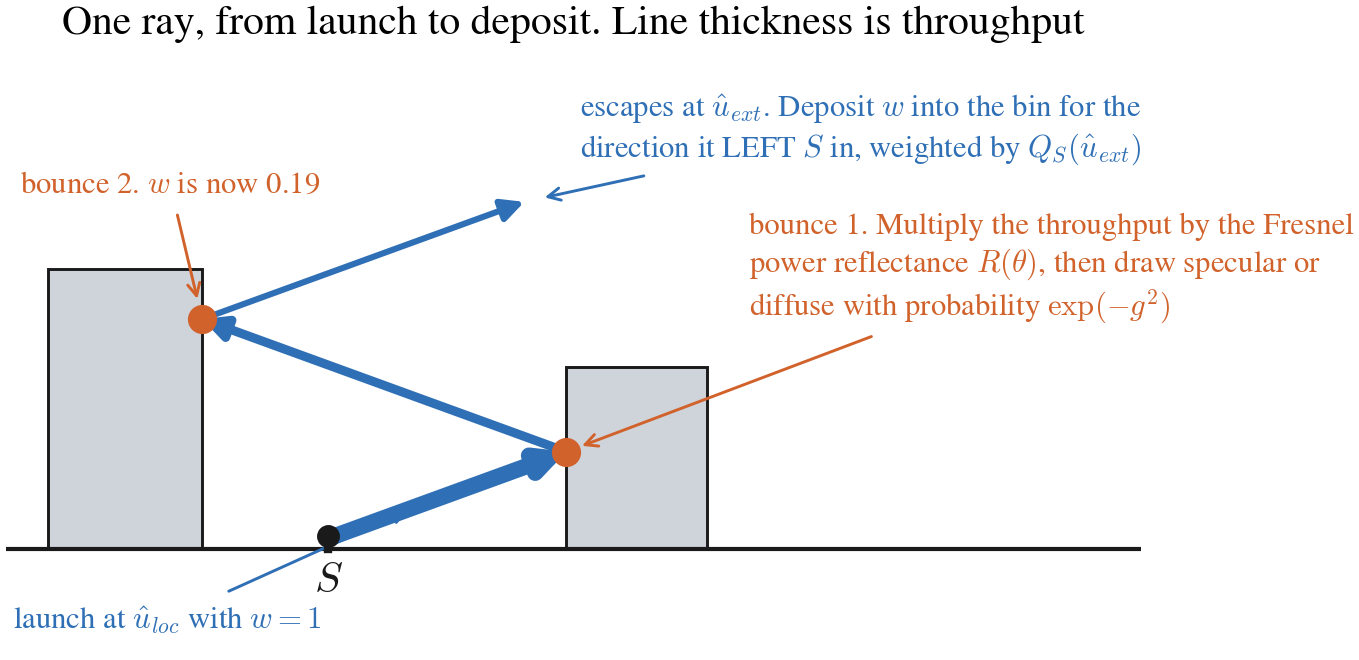
\includegraphics[width=\columnwidth]{21_one_ray.pdf}
  \caption{One ray leaving the head, reflecting twice off facades and escaping
  to the sky. Line thickness is the surviving power $w$. The ray deposits
  $w\,Q(\uext)$ into the angular cell it was launched into, not the one it
  escaped through.}
  \label{fig:oneray}
\end{figure}

\subsection{Quantities that come for free}

Three diagnostics fall out of the same trace at no extra cost. The sky fraction
is the share of rays that escape without touching anything, which is the solid
angle of open sky above the standpoint. The direct exposure ratio uses only
those same rays, so the ratio of $\chi$ to it measures how much the surroundings
add by reflection. The mean excess path length, taken over escaping rays
weighted by their power, gives the delay spread the square would impose. All
three are reported alongside $\chi$.

\section{Body coupling}

The trace gives the power arriving at $\x$ from each direction. Turning that
into absorbed power on a body is a separate calculation and is done with an
established phantom and tissue model rather than reimplemented here
\cite{aegis, itis}. For a facet with outward normal $\nhat$ under a plane wave
travelling along $\khat$,
\begin{equation}
  S_{ab} = S_{\mathrm{inc}} \, T_0 \, \max\!\left[ \nhat \cdot (-\khat),\, 0
  \right] ,
  \label{eq:sab}
\end{equation}
where $T_0$ is the power transmitted into skin at normal incidence at 15\,GHz
and the clamp removes facets that face away. The arriving distribution
$\Phi(\uloc)$ is passed in as a set of plane waves, one per angular cell, with
the direction dictionary $\khat = -\uloc$ that reciprocity requires. Summing
\eqref{eq:sab} over cells gives the absorbed power density map on the body, and
integrating that map gives the absorbed power and the whole body specific
absorption rate. Two things are left out of this step. The phantom stands alone,
so other people nearby, who would block part of the near horizon at the same
height as the head, are absent. The body is also treated as convex, so one limb
never shadows another, which matters most for arrivals that graze along the
body.

\section{Validation}
\label{sec:valid}

The estimator is checked in three ways, ordered from those that need no
reference value to those that need a reference calculation.

\subsection{Identities}

Some results follow from the construction and must come out exactly. Under the
isotropic model $\chi$ must equal the sky fraction, because weighting all
directions equally means the answer is the open solid angle and nothing else,
and the two are computed by different code paths. In an empty scene every model
must return $\chi = 1$. Reversing every path must leave the transported power
unchanged. Total reflected power must never exceed incident power at any
interaction. These are property tests over randomised inputs rather than single
cases.

\subsection{Closed forms}

Two geometries have analytic answers. A single infinite ground plane below the
standpoint gives a $\chi$ that can be written down from \eqref{eq:cone} and the
Fresnel coefficient alone. A Lambertian spherical cavity gives a second, with a
different balance between the direct and the multiply reflected contribution.
Both are reproduced to the tolerance set by the ray count.

\subsection{Convergence}

Three parameters are measured rather than chosen. The number of surface
interactions $L$ is raised until the median change in $\chi$ falls below
0.5\,dB. That comparison needs one remark, because the obvious way to read it is
wrong. Two runs that differ only in $L$ and share a seed trace the same rays and
agree exactly up to the shallower depth, so their difference is paired and is
resolved far better than either value is on its own. Reading it against the
single run error of the next paragraph would make a real and well measured
difference look like noise. The ray count $N$ is raised until the spread across
independent seeds falls below the differences being interpreted. The crop radius is raised until
$\chi$ stops moving, which is what fixes the 250\,m figure quoted in
Section~II: at smaller radii the mesh is missing buildings that would have
blocked near horizon paths, and the near horizon is where the illumination
models put most of their measure. The converged radius is a property of the
illumination model and not of the site, so it is reported per model.

Identities and closed forms constrain the implementation, not the formulation.
A derivation error that is coded faithfully passes all of them, and one such
error was in fact found by rederiving \eqref{eq:cone} rather than by any test
failing. An independent solver is therefore used as an external check, and the
comparison is reported with the results.

\begin{thebibliography}{9}

\bibitem{itu2040}
International Telecommunication Union, ``Effects of building materials and
structures on radiowave propagation above about 100 MHz,'' Recommendation
ITU-R P.2040-4, 2023.

\bibitem{beckmann}
P.~Beckmann and A.~Spizzichino, \emph{The Scattering of Electromagnetic Waves
from Rough Surfaces}. Oxford, U.K.: Pergamon, 1963.

\bibitem{arvokirk}
J.~Arvo and D.~Kirk, ``Particle transport and image synthesis,'' in
\emph{Proc. SIGGRAPH}, 1990, pp. 63--66.

\bibitem{aegis}
R.~Wydaeghe, ``AEGIS: absorbed power density on human bodies in wireless
environments,'' software, 2026.

\bibitem{sam}
A.~Kirillov \emph{et al.}, ``Segment anything,'' in \emph{Proc. IEEE/CVF Int.
Conf. Comput. Vis.}, 2023, pp. 4015--4026.

\bibitem{itis}
P.~A.~Hasgall \emph{et al.}, ``IT'IS database for thermal and electromagnetic
parameters of biological tissues,'' Version 4.2, 2024.

\end{thebibliography}

\end{document}
